\note{
Perm-iso in kanonische Gestalt rekonstruieren.
Dann Klassifikation endlicher einfacher Gruppen anwenden.

Typ PA: einfachster nicht-trivialer Fall.
}

\begin{frame}{Schwach kanonische Form (1)}
\begin{block}{Typ PA}
Sei $G \leq \sym \Omega$ eine primitive Gruppe vom Typ PA.
\pause
Dann ist $G$ in \emph{schwach kanonischer Form}, falls
eine einfache Gruppe
$T \leq \sym \Delta$
existiert,
so dass
$\Omega = \Delta ^ \ell$ und
$\soc G = T ^ \ell \leq \sym( \Delta ^ \ell)$ ist.
\end{block}

\pause
\begin{block}{Satz}
$G$ wie oben. Dann kann
\[
    N_{\sym (\Delta ^ \ell)}(\soc G) =
    N_{\sym \Delta}(T) \wr S_\ell
\]
in polynomieller Zeit berechnet werden.
\end{block}
\end{frame}

\begin{frame}{Schwach kanonische Form (2)}
\begin{block}{Typ PA}
Sei $G \leq \sym \Omega$ eine primitive Gruppe vom Typ PA.
Dann ist $G$ in \emph{schwach kanonischer Form}, falls
eine einfache Gruppe
$T \leq \sym \Delta$
existiert,
so dass
$\Omega = \Delta ^ \ell$ und
$\soc G = T ^ \ell \leq \sym( \Delta ^ \ell)$ ist.
\end{block}

\pause
\begin{block}{Satz}
Sei $G \leq \sym \Omega$ eine primitive Gruppe. Ein Permutationsiso. in schwach
kanonische Form kann in Las Vegas fast-linearer Zeit
und in deterministisch polynomieller Zeit
berechnet werden.
\end{block}
\vspace{2em}
\end{frame}

\note{das Beste zum Schluss.
Jeder der mal was mit Permutationsgruppen zu tun hatte, weiß, dass diese
schnell "messy" werden können.
Um WCF zu berechnen benutzen wir perm mors.


Motivation:
1. Für PA Typ: Wir schreiben $\soc G$ als \emph{Produkt} in einer geeigneten
Kategorie.

2. Ein Permutationsiso ist eindeutig durch die Gruppe $G$ und die
Punktabbildung $f : \Omega \to \Delta$ gegeben.

Also sollte es ausreichen $\Omega$ in $\Delta ^ \ell$ zu zerlegen.}

\begin{frame}{Permutationsmorphismen}
Seien $G \leq \sym \Omega$, $H \leq \sym \Delta$ Gruppen
mit den natürlichen Operationen
$\rho_G$ und $\rho_H$
\pause
und
seien
$f : \Omega \to \Delta$, $\phi : G \to H$.
\pause
Das Paar $F = (f, \phi)$ heißt
\emph{Permutationsmorphismus von $G$ nach $H$},
falls
\[
\begin{tikzcd}[ampersand replacement=\&]
    \Omega \times G
        \ar[r, "\rho_G"]
        \ar[d, "f \times \varphi"]
    \&
    \Omega
        \ar[d, "f"]
    %
    \\
    %
    \Delta \times H
        \ar[r, "\rho_H"]
    \&
    \Delta
\end{tikzcd}
\]
kommutiert.

\pause
\begin{block}{Satz}
Permutationsgruppen zusammen mit Permutationsmorphismen und ``vertikaler''
Verknüpfung bilden eine Kategorie $\mathbf{PermGrp}$.
\end{block}
\end{frame}

\note{
Falls Zeit ist:
Jede Permutationsgruppen kann als Kategorie, nämlich als Gruppoid, modelliert
werden.
$\Omega$ ist Menge der Objekte.
$Mor(\alpha, \beta) = \set{ g \in G ~|~ \alpha ^ g = \beta }$.

Permutationsmorphismen sind dann Funktoren zwischen diesen Gruppoiden.
}

\begin{frame}{Permutationsmorphismen: Produkte (1)}
\begin{block}{Satz}
$\mathbf{PermGrp}$ enthält alle endlichen Produkte.
\end{block}
\end{frame}

\begin{frame}{Zusammenfassung}
Der Algorithmus:
\begin{itemize}
\item Schwach kanonische Form
\item Normalisator des Sockels
\item Logarithmische Reduktion
\item $2 ^ {O(n)}$ Algorithmus von Wiebking
\item Urbild unter der Reduktion
\end{itemize}
\end{frame}

\begin{frame}[standout]
Danke!
\end{frame}

\note{
Abschließende Worte?
Wie zurück vom Detaillierten zum großen Ganzen?
}

\begin{frame}{Permutationsmorphismen: Produkte (2)}
\begin{block}{Beispiel}
$\Omega := \set{1, \ldots, 4}$ und
$V := \langle a := (1,2)(3,4),~$%
$b := (1,3)(2,4) \rangle$.

\begin{figure}[H]
\centering
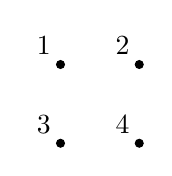
\begin{tikzpicture}
    % nodes
    \foreach \x in {1, ..., 2}
        \foreach \y in {1, ..., 2}
            \draw [fill] (\x, \y) circle [radius=0.050];
    \node [above left] at (1, 2) {{$1$}};
    \node [above left] at (2, 2) {{$2$}};
    \node [above left] at (1, 1) {{$3$}};
    \node [above left] at (2, 1) {{$4$}};
\end{tikzpicture}
\end{figure}

Ferner sei
$P_1 := (p_1, \pi_1)$ mit
\begin{align*}
p_1 &: \Omega \to \set{1,3},~~
1,2 \mapsto 1, ~~ 3,4 \mapsto 3,
\\
\pi_1 &: G \to \gen{(1,3)},~~
\id_\Omega, a \mapsto \id_{\set{1,3}},
~~b, ab \mapsto (1,3).
\end{align*}

Analog $P_2$.
Dann $P_1 \times P_2 : V \iso \gen{(1,3)} \times \gen{(1,2)}$
\end{block}
\end{frame}

\begin{frame}{Permutationsmorphismen: Produkte (3)}
\begin{block}{Satz}
Sei $G \leq \sym \Omega$.
Für $i = 1, \ldots, \ell$
seien
$(p_i : \Omega \to \Omega_i)$
mit $G$ kompatible Abbildungen,
\pause
die mit $\Omega$ ein Produkt in
$\mathbf{Set}$ bilden.
\pause
Ferner seien
$P_i = (p_i, \pi_i)$ die eindeutigen ``Fortsetzungen'' der $p_i$ zu
Permutationsepimorphismen
von $G$.
\pause
Dann gilt
\[
G \text{ bildet mit } (P_i)_{i \leq \ell} \text{ ein Produkt }
\iff
\prod \pi_i \text{ ist Epim. }
\]
\end{block}
\end{frame}
